\section{Gestión de Médicos Asociados}
Una de las herramientas más innovadoras que ofrecemos es la capacidad de digitalizar tus reportes y enviarlos automáticamente a tus médicos privados. Este proceso preserva tu privacidad, obligando a que tú seas el único que pueda autorizar la lectura a los especialistas de tu confianza.

\subsection{Buscar y Conceder Acceso}
Para darle acceso a tu médico de cabecera a todos tus resultados pasados, presentes y futuros:
\begin{enumerate}
    \item En el menú superior (o lateral) de tu Dashboard, haz clic en la sección \textbf{"Mis Doctores"}.
    \item Llegarás a una pantalla con un buscador en la parte superior con el texto "Buscar por nombre...".
    \item Haz clic en la caja de búsqueda y teclea el \textbf{nombre completo} de tu médico tratante para filtrarlo.
    \item El sistema abrirá un menú desplegable interactivo por debajo de tu búsqueda evidenciando a los doctores de nuestra red de prestadores que concuerden con las letras tecleadas y que tengan su licencia legal vigente y certificada.
    \item Cuando ubiques la tarjeta del profesional correcto (te sugerimos revisar su universidad y cédula), haz clic explícitamente en el pequeño botón verde claro rectangular a la derecha que dice \textbf{"+ Agregar"}.
    \begin{figure}[H]
        \centering
        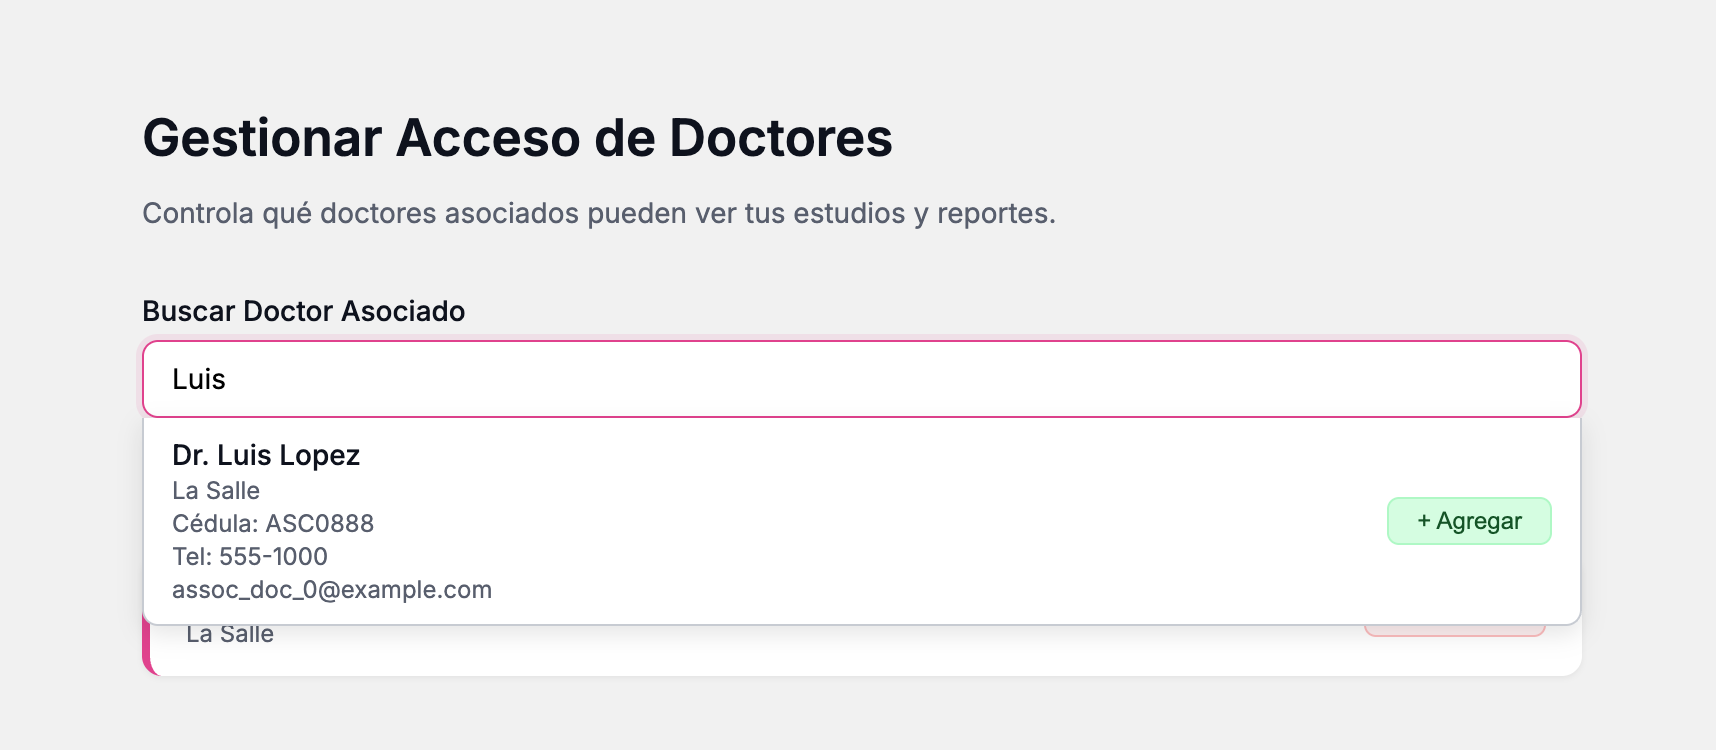
\includegraphics[width=0.5\linewidth]{screenshots/doctor_search.png}
        \caption{Ejemplo de la herramienta de busqueda.}
    \end{figure}
    \item Aparecerá un mensaje verde claro de "Acceso concedido" (notificación \textit{toast}) en la esquina inferior derecha de tu aplicación. 
    \item La tarjeta de dicho médico bajará a la sección inferior de tu pantalla titulada "Doctores con Acceso". A partir de ese momento, el doctor cuenta con visualización compartida irrestricta a tu historial de PDFs radiológicos desde su propia cuenta. (El sistema bloquea la descarga de reportes para el doctor, en caso de revocación de permiso, el doctor dejará de tener acceso a tu historial médico.)
    \begin{figure}[H]
        \centering
        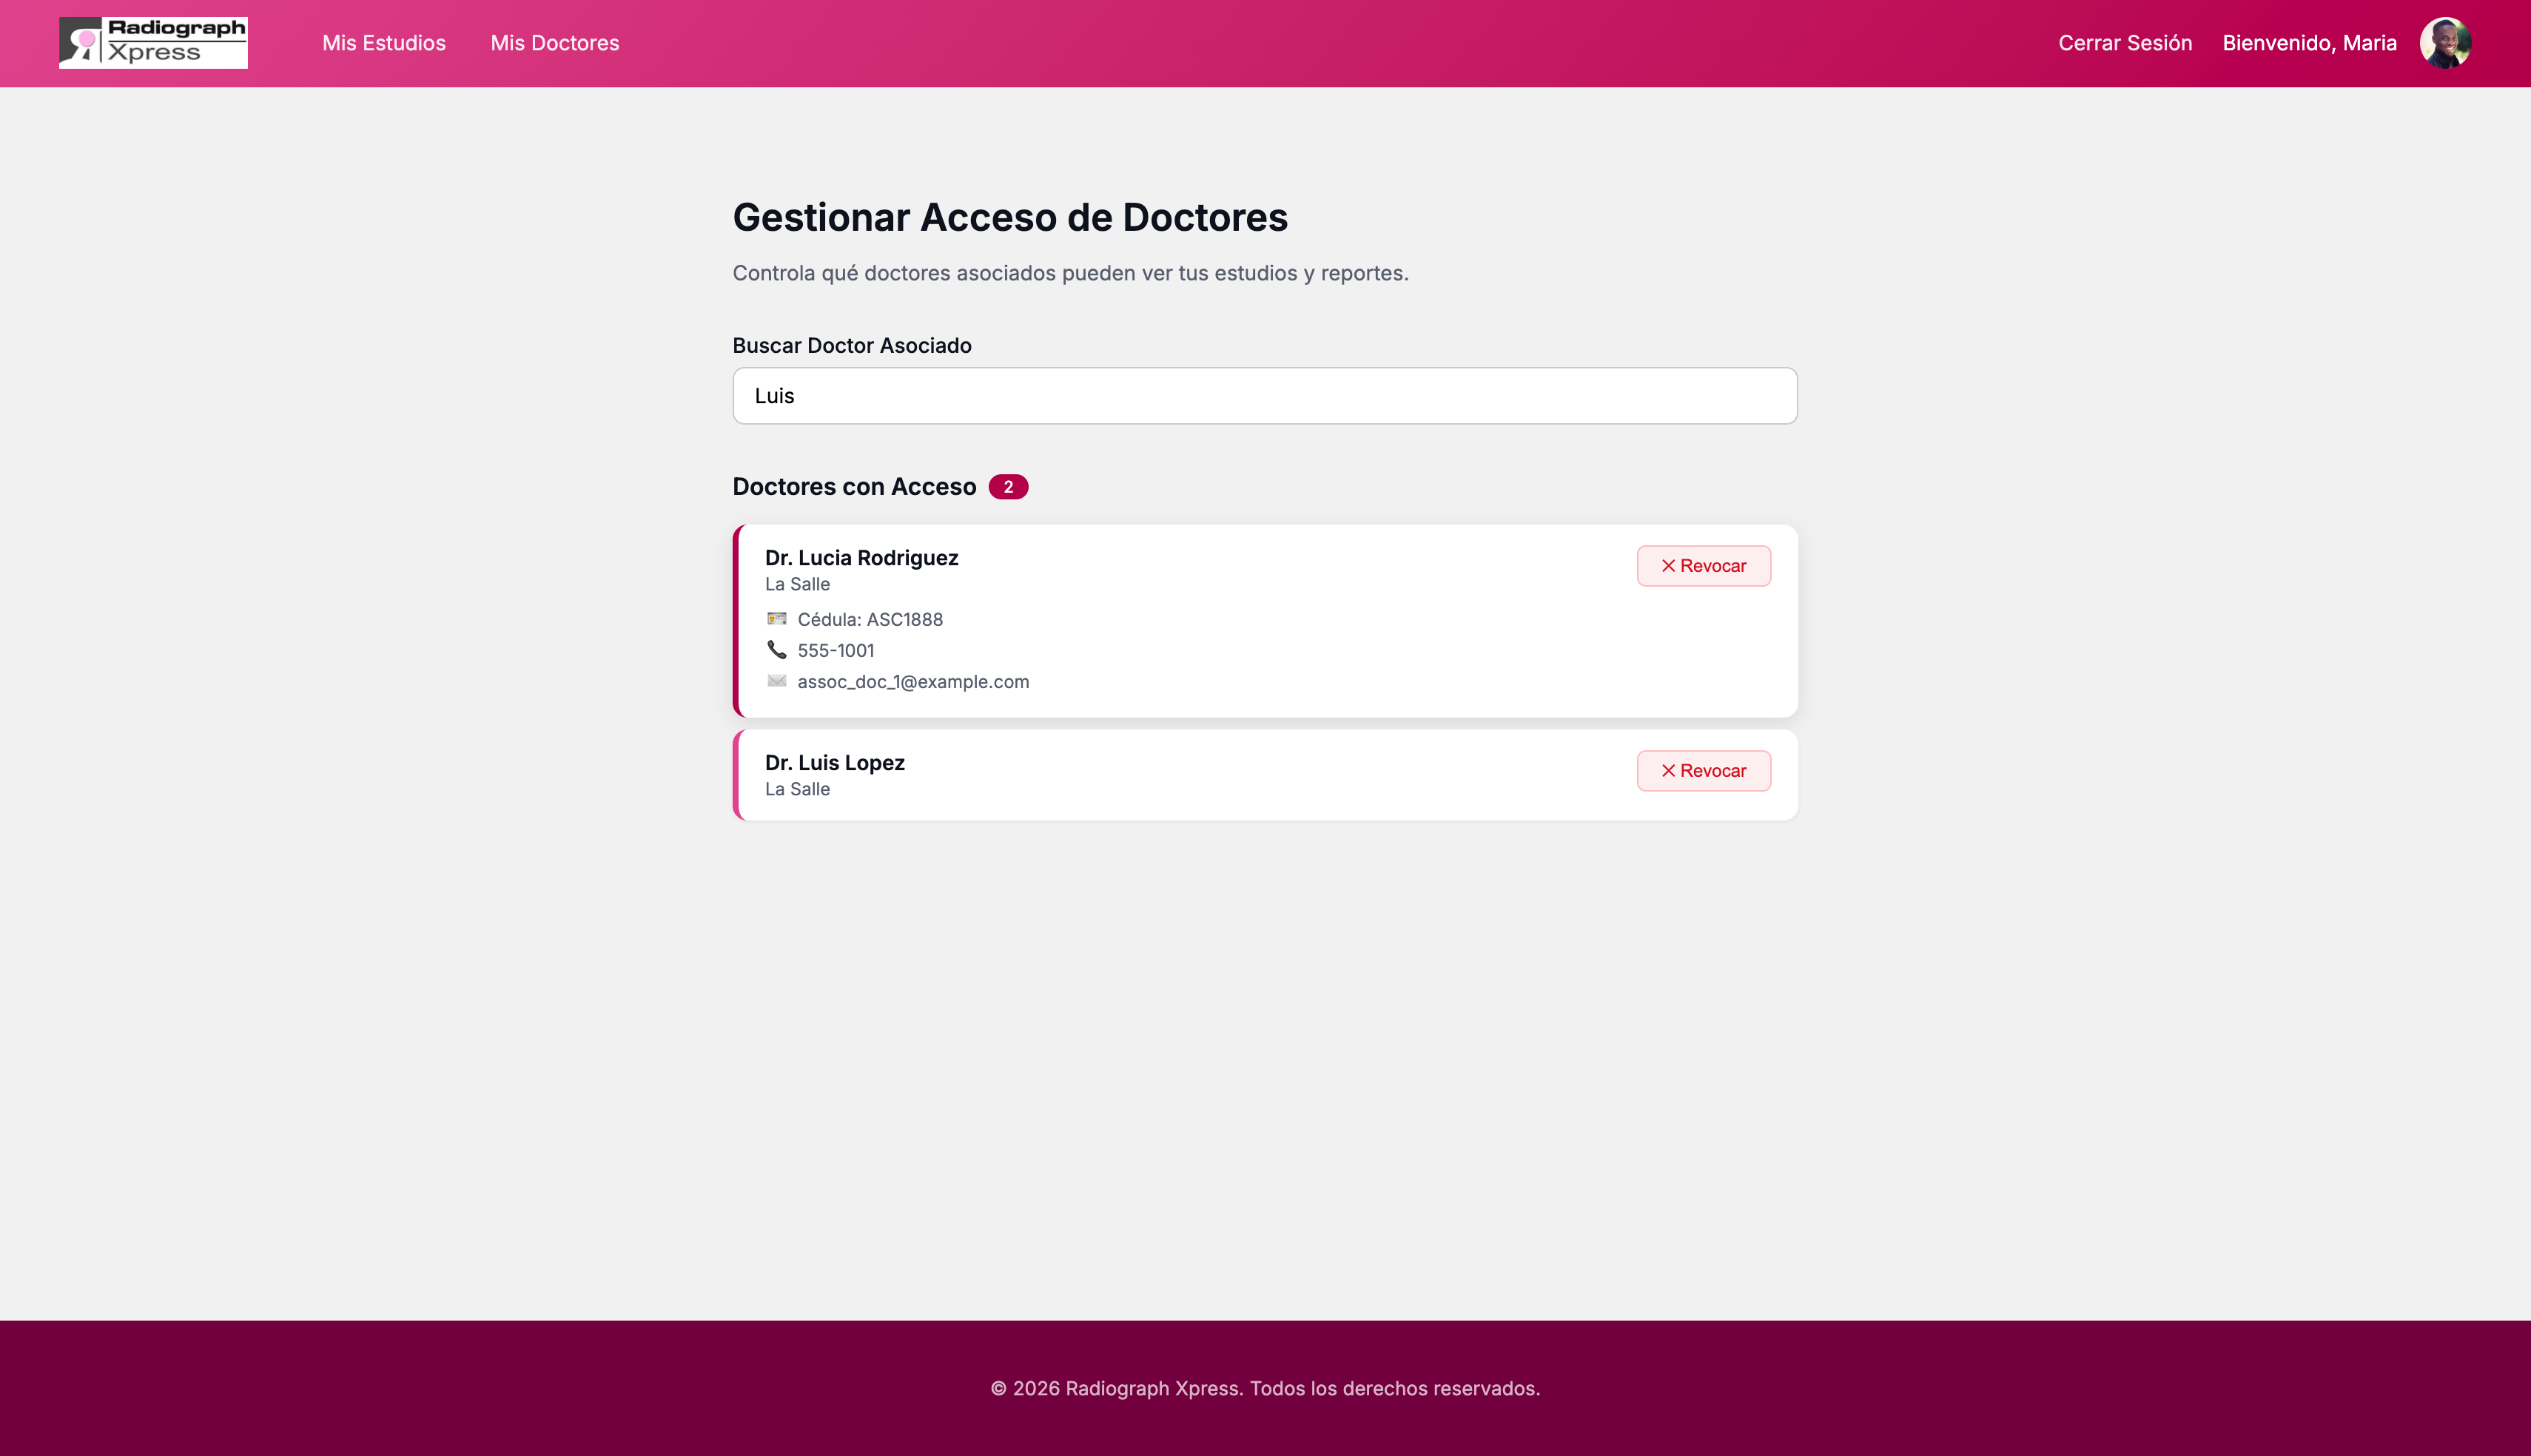
\includegraphics[width=0.5\linewidth]{screenshots/allowed_doctors.png}
        \caption{Ejemplo de doctores con autorización.}
    \end{figure}
\end{enumerate}

\subsection{Revocación Expeditiva}
Nuestros estándares corporativos de privacidad te otorgan absoluto control y soberanía sobre la administración de tus datos de salud. Tienes la libertad legal de revocar el permiso de cualquier especialista, en el instante en que lo desees, sin emitir ningún aviso previo.
\begin{enumerate}
    \item En la misma página de `Mis Doctores`, desplaza la pantalla hasta llegar a visualizar la división "Doctores con Acceso".
    \item Podrás ver una lista de tarjetas de recuadros blancos con todos los doctores vinculados vigentes. A la derecha de cada tarjeta, observarás un botón rojo marcado con el texto \textbf{"X Revocar"}.
    \item Ubica al médico con el que dejarás de tener relación clínica y presiona este botón sobre su tarjeta.
    \item En cuestión de milisegundos, el sistema procesará la instrucción a nivel de base de datos; visualizarás cómo su tarjeta es barrida y eliminada en vivo ante tus ojos y recibirás una notificación de "Acceso revocado".
    \item Con esto, inmediatamente se le revocarán las claves y los identificadores, por lo que todo rastro de tu expediente desaparecerá herméticamente de su portal sin vuelta atrás.
\end{enumerate}
